\documentclass[11pt,a4paper]{article}
\usepackage[latin1]{inputenc}
\usepackage{amsmath}
\usepackage{amsfonts}
\usepackage{amssymb}
\usepackage{graphicx}
\usepackage{tabulary}
\usepackage{multirow}
\usepackage{setspace}
\usepackage{booktabs}
\usepackage{longtable}
\usepackage{natbib}
\usepackage{csquotes}
\let\oldenquote\enquote
\renewcommand{\enquote}[1]{{\itshape\oldenquote{#1}}}
\usepackage[top=1in, bottom=1.25in, left=1.25in, right=1.25in]{geometry}
%\singlespacing
\onehalfspacing


\author{Stefan K\"uhn\thanks{International Labour Organisation, kuehn@ilo.org}  and Sheena Yoon\thanks{International Labour Organisation, yoons@ilo.org}}
\title{Women's participation in the labour market around the world: life-cycle effects of preferences, gender norms and socio-economic constraints\thanks{The information and views set out in this paper are those of the authors and do not necessarily reflect the official opinion of the ILO.}}
\date{\today\\
	\texttt{Working Paper}}


\begin{document}
\maketitle
\abstract{This paper relates the probability for women to participate in the labour market to a complex framework of fundamental drivers, covering socio-economic constraints, gender role conformity and personal preferences. The validity of the framework is verified empirically using the 2016 Gallup World Poll, a rich survey dataset covering individuals in 127 countries with an identical questionnaire. Importantly, the dataset includes new indicators of personal preferences, societal gender norms and socio-economic constraints developed by the International Labour Organization (ILO) and administered in the survey to specifically capture the three driving influences on women's participation. First, by using the age dimension of the dataset the paper finds that the fundamental drivers differ in their impact depending on the life-cycle situation women are in. Second, with the help of the unique cross-country dimension of the dataset the paper establishes that their impact also differs by country characteristics. 
}

\section{Introduction}
The past couple of decades has been marked by economic transformation, demographic change, declining fertility, technological progress, advancement in education and health, and shifts in social norms that has in many ways helped women enter the labour force around the world.  Yet, despite a backdrop of economic, social, and political transformation, the gender gap in labour force participation continues to persist at 27 percentage points and the participation rates of women has endured a slowdown in the past decade. This suggests that globally, we are still far away from closing the gender gap as women continue to face a multiplicity of constraints restricting their capabilities and freedom to access the labour market.  

A recent joint ILO-Gallup survey demonstrates that women are clearly facing multiple constraints when the majority of women (70 per cent) prefer to work a paid job while approximately half of women globally still remain out of the labour force. Even among those out of the labour force, their preference to work remains a majority at 58 per cent. Ensuring that all women who have the preference to work can freely do so, equally as men, increases their autonomy in the household and in the public domain while contributing to other dimensions of gender equality (Kabeer 2002, 2004; Elson 1999). Yet, not all decisions to participate are freely made when women under economic constraints have no choice, but to work out of necessity, while often carrying the double burden of both unpaid and paid labour. Moreover, increased participation does not necessarily imply that women are better off considering that they are overrepresented in low-paid and labour-intensive sectors and occupations with sub-optimal working conditions, which may simultaneously discourage participation (Kucera and Tejani, 2014, Cagatay and Ozler 1995). 

Alternatively, for certain groups of women, the trade-off of participation for higher education or retirement can be a more desirable and preferred opportunity. Hence, women around the world not only face various drivers and constraints to participation but, how their preference and decision to participate are affected depends on their position in their life-cycle (\cite{besamusca2015working}). For instance, prime-age working women often face greater care demands when married and with younger children than youth or older women.

As a result of the findings of the recent ILO-Gallup survey, on women's preferences and their life evaluations associated with the labour market, this paper contributes to the ongoing discussion of female labour force participation by analysing which factors constrain or drive participation and to what extent in the life-cycle. The paper expands previous work in two important dimensions. First, it utilizes the results from newly developed survey questions by the International Labour Organization (ILO) designed to specifically identify personal preferences of women, societal and household acceptability of women working, and the life-evaluation of women in the labour market. This motivates the paper to address the following questions: (i) to what extent is the decision to participate driven by individual preferences? (ii) how do gender roles shaped by social norms affect participation? (iii) to what extent do socio-economic constraints affect participation? and (iv) how do these socio-economic constraints differ according to the life-cycle? Second, the ILO survey questions administered within the 2016 Gallup World Poll, creates an immensely rich dataset covering 149,000 adults in 142 countries, thereby representing 99 per cent of the global adult population and providing the opportunity to study the labour participation of women across all income and cultural groups. Moreover, this paper employs a life-cycle analysis by distinguishing different age groups (youth, prime-age working, 55+) to account for the life-cycle effects on women's participation to consider the different drivers or constraints women face at different points in their life. 

In Section~\ref{sec:framework}, we review the relevant literature and construct a conceptual framework of the fundamental drivers of female labour force participation.  Section~\ref{sec:data} summarizes the dataset and Section~\ref{sec:methodology} presents the empirical methodology. Section~\ref{sec:results} reports the results. Section~\ref{sec:conclusion} concludes and discusses the  potential research subsequently arising from the paper's findings.
 
\section{A conceptual framework of labour market outcomes}\label{sec:framework}
A woman's decision whether to participate or not in the labour market involves a complex set of fundamental drivers in conjunction with life-cycle circumstances, which can be broadly classified as (i) personal preferences, (ii) socio-economic constraints, and (iii) gender role conformity (Figure~\ref{fig:framework}). These three fundamental drivers are conditional on or are determined by the prevailing gender social norms in the society that a woman inhabits.

\begin{figure}[htb]
	\centering
	\caption{Conceptual framework}
	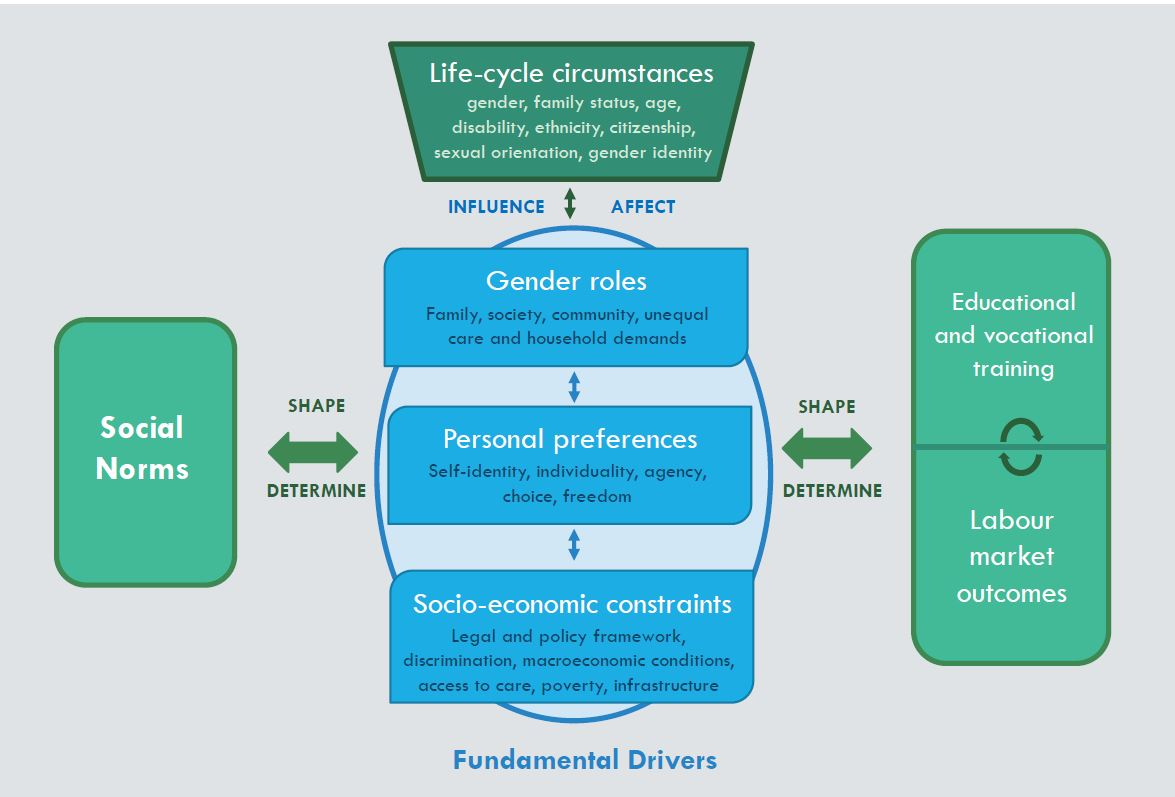
\includegraphics[width=120mm,keepaspectratio,height=0.6\textheight]{Figures/framework_1}
	\label{fig:framework}
\end{figure}

Personal preferences are an important driver of an individual's labour market outcome, within the constraints set by prevailing social norms and socio-economic factors (in conjunction with life-cycle circumstances) (figure 5). Indeed, a woman's preference for engaging in work is an expression of both what is perceived to be legitimate in her personal circumstances and her socialized identity (\cite{ilogallup2017} and Sen, 1987). In fact, many women who prefer to work, are able to choose to do so and, as result, derive pleasure and economic and social well-being from decent work opportunities. On the other hand, some women may prefer to stay at home due to a lack of jobs that are "socially acceptable" for women, because childcare costs may exceed their potential incomes or because their role within the household may be perceived as more valuable (economically and socially). However, personal preferences are also shaped by what is perceived to be legitimate and accessible, and are hence endogenous to gender norms and socio-economic constraints (\citet*{sen1995agency}).
 
Socio-economic constraints represent the institutional, economic and physical constraints faced by both men and women. As discussed above, economic conditions can dictate the availability and quality of jobs, both within and across countries. For instance, a downturn in the business cycle can temporarily provoke economic necessity within a household, in which case women often move into paid employment, so that, in effect, their labour supply acts as an insurance mechanism (Attanasio, Low and Sánchez-Marcos, 2005; Bhalotra and Umana-Aponte, 2010). Among institutional constraints, the legal and policy framework of tax systems can often impose high marginal tax rates on secondary earners with lower income, who are more likely to be women, hence disincentivizing their participation in the labour force (Stotsky, 1996; \cite{Jaumotte2003}; EC, 2015). Alternatively, the lack of care facilities poses a problem for the entire household, but in reality its effect is disproportionally felt by women due to their assigned gender role as caregivers (\cite{badgett1999assigning}). Additionally, discrimination directly creates gender gaps through the disadvantageous treatment of women in terms of payment, hiring or promotion. Importantly, since policy is, at least in part, a function of and influenced by gender social norms, it is influential in shaping the extent of socio-economic constraints and the magnitude of their effects while simultaneously reinforcing existing gender prevailing norms (Sjoberg, 2004).
  
Gender role conformity arises from traditional gender social norms that operate at multiple levels   of society, ranging from religion to economic class, race and locality. Class, patriarchy and social hierarchy, often determined by caste, ethnicity and religion, interact with one another to shape society's norms around gender roles (\cite{bardhan1984land}; \cite{klasen2012push}). As a result, women are often compelled to conform to the gender roles deemed to be acceptable by their family, community or society in order to avoid the consequences of social exclusion, insecurity or other conflicts. These attitudes towards gender roles construct a social hierarchy that not only defines women's roles in the labour market, but also adds to the disproportionate burden of household responsibilities that they must bear (Badgett and Folbre, 1999).

The three fundamental drivers as described above help determine the various labour market outcomes of women, notably (i) labour market participation, (ii) occupation or sector of employment, (iii) type of employment relationship, and (iv) income. This relationship, however, is recursive. The labour market outcomes themselves can influence the decision to participate in the labour market in the first instance. Put simply, unequal labour market outcomes (e.g. if women are paid less or have limited occupational opportunities) can shape the decision to participate. 

In addition, these labour market outcomes are interdependent. For example, if due to social norms women can only find employment in certain types of occupations that are characterized by part-time employment relationships and lead, in turn, to a wage penalty, then occupation, employment type and income are reinforcing one another.

Related is the importance of education. Educational opportunities (including access and quality) are affected by social norms. Indeed, gender differences in most developed countries can manifest themselves in the choice of study and in developing and emerging countries the level of education that is achievable (EC, 2009). In this respect, education, including vocational training, is a primary determinant of labour market outcomes. Moreover, educational attainment and the field of study determine not only labour market entry but also career trajectories (then affect other aspects of the labour market such as occupational choice and income). 

As evidenced by the discussion, there is a considerable level of inter-connectivity and inter-dependence among the drivers and labour market outcomes. With this in mind, the next section identifies and isolates - to the extent possible - the impact of these individual drivers on female labour force participation rates. The approach therefore links to the  "capabilities approach"  by capturing the voices of women expressing the challenges they face within the labour market, their preferences in terms of work, their perception of their own futures and the normative constraints on their agency which they face. Hence, this analysis strives to capture the empowerment, agency and ability of women to make decisions, both within the home and in the labour market.

\section{Data description}\label{sec:data}

The principal data source is the 2016 instalment of the Gallup World Poll. This is a survey undertaken by Gallup, where 149 thousand persons in 142 countries have been asked an extensive set of questions on a whole range of issues. Table~\ref{tab:vardescription} presents the questions that have proven to be of relevance for explaining female labour force participation. Due to missing data in some countries, the sample is reduced to 60126 women in 121 countries.

Importantly, no observations are dropped within countries that form part of the analysis, the sample reduction affects complete countries. Hence, the estimated results are unbiased for the countries under analysis. Given that 121 countries is still a very large sample, and that missing countries tend to be rather small, obtained results can be generalized.


\begin{longtable}{|p{0.3\textwidth}|p{0.1\textwidth}|p{0.6\textwidth}|}
%	\centering
	\caption{Description of variables}\label{tab:data_descr}\\
	\hline
		\textbf{List of variables}& \textbf{Symbol} & \textbf{Description} \\
		\hline
		\endfirsthead
	\caption{continued...}\\
		\hline
		\textbf{List of variables} & \textbf{Symbol} & \textbf{Description}  \\
		\hline
		\endhead
		\hline
		\endfoot
		Age &$AGE$ & Young (15-24) \\
		&& Prime age (25-54) \\
		&& Old (55+)\\
		\hline
		Children &$CHD$ & Dummy if having at least one child\\
		\hline
		Household members &$HHM$ & Actual numeric value \\
		\hline
		Education &$EDU$  & Primary education (base level) \\
		&& Secondary education \\
		&& Tertiary education \\
		\hline
		Relationship &$RLS$ &Single, widowed, separated or divorced (base level) \\
		&& Married, living with partner\\
		\hline
		Internet, Phone, Communication & $INT$, $PHO$, $COM$ & Dummy for having access to internet or phone (mobile or landline), or both \\
		\hline
		Urban &$URB$ & Rural (base level), urban \\
		\hline
		Poverty &$PVT$ & No poverty (base level)\\
		&& Mild poverty (not enough money for either food or shelter) \\
		&& Severe poverty (not enough money for food and shelter) \\
		\hline
		Religion &$REL$ & Secular/atheist (base level) \\
		&& Other \\
		&& Christian \\
		&& Muslim \\
		&& Hindu \\
		\hline
		\multirow{1}{0.3\textwidth}{Question "Do you prefer to work in a paid job, stay at home, or do both"} &$PFW$& Response: \\
		&& "Stay at home" (base level)\\
		&& "prefer paid job" or "both" \\
		\hline
		Acceptability of paid work &$ACW$ & Dummy, women answering that household members find it acceptable for a women to work in a paid job. \\
		\hline
		Opportunity (better, worse) &$OPP$ & Dummy when person finds that women have better (worse) opportunity on labour market than men given equal education, base level same opportunity. \\
		\hline
		Job climate index &$JCL$ & Continuous, an index (values 0, 50, 100) computed by Gallup capturing the perceived labour market environment by a respondent.  \\
		\hline
		Roads &$RDS$ & Dummy, whether respondents are satisfied (1) or dissatisfied with the road infrastructure in their environment\\
		\hline
		Law and order &$LAW$ & Continuous, an index (7 levels) from Gallup capturing how respondents view the state of law and order.\\
		\hline
		\multirow{1}{0.3\textwidth}{Major challenge faced in labour market:} &$CHG$ & Lack of flexible work hours (base level)\\
		&& Balance between work and family or home\\
		&& Lack of affordable care for children or relatives\\
		&& Family members don't approve of women working\\
		&& unfair treatment at work/abuse/harassment/discrimination\\
		&& Lack of good-paying jobs\\
		&& Unequal pay for doing similar work as men\\
		&& Lack of transportation/lack of safe transportation \\
		&& People prefer to hire or promote men\\
		&& Lack of skills, experience or education
	\label{tab:vardescription}%
	\end{longtable}%

The survey contains basic information about respondents such as their age, sex, family status, education level and religion. Next, some questions cover the labour market status of respondents. Furthermore, questions relate to the environment in which subjects live, revealing for example their household size, the number of children in the household, whether they live in an urban or rural environment and the availability of communication devices in the home. Frequently, the survey also contains questions on household income. However, the 2016 instalment did not cover this, containing only questions on whether households lack money for food or shelter, respectively, which serves as an indicator of poverty. 

Also, the survey contains a large number of questions about the opinion of respondents on certain issues, such as how favourable they see the United States. The most interesting of these opinion questions for the purposes of this analysis is the job climate index, which shows how respondents evaluate the current prospects for jobs in their environment.

Finally, the 2016 instalment of the Gallup World Poll covers a number of questions designed by the ILO in order to identify the opinion of women and men about women's position in the labour market. A detailed analysis of these opinions has been published in \citet{ilogallup2017}. Four of these questions are of importance for this paper. 

The first one asks women \enquote{Would you PREFER to work at a paid job, or stay at home and take care of your family?} The choices were either \enquote{Work at paid job}, \enquote{Stay at home} or \enquote{Both}. The second question asked \enquote{It is perfectly acceptable for any woman in your family to have a paid job outside the home IF SHE WANTS ONE. Do you agree?} The answering choices were \enquote{Agree} or \enquote{Disagree}.

The third question asked \enquote{Please think about women who work at paid jobs in [country/territory name] today. What do you think is the BIGGEST challenge these women face?} Responses were unprompted, and then coded into one of ten categories (see table~\ref{tab:vardescription}). The fourth question asked was \enquote{If a woman has similar education and experience to a man, does she have a better opportunity, the same opportunity, or a worse opportunity to find a good job in the city or area where you live?} All of the questions could also be answered with \enquote{Don't know}.

Country-level information is retrieved from other sources. The labour force participation rates for women are taken from ILOSTAT. The GDP per capita, as well as the country classification into income categories, is taken from the World Bank's World Development Indicators.


\section{Empirical methodology}\label{sec:methodology}

The aim of the empirical analysis is to find relevant  factors explaining women's labour force participation, and to compare their impact across different groups of women identified by the research questions at hand. The  variables available for analysis have been described in the previous section.

\subsection{Econometric model}
The variable of interest, labour market participation, is a binary variable. The econometric model of choice in such a case is to estimate the probability of a woman to participate in the labour market, depending on explanatory variables, using a probit specification. 

In such a model, the probability of a woman to participate, $Pr(P=1)$, depending on a set of explanatory variables $X$, is modelled using the cumulative distribution function of the standard normal distribution ($\Phi()$). 
\begin{equation}\label{eq:estimation}
Pr(P=1|X) =\Phi\left(X^T \beta \right)
\end{equation}
This function is bound between zero and one and is solved using maximum likelihood techniques.

The theoretical framework established that the fundamental drivers of labour market outcomes are in fact also shaped by the labour market outcomes themselves. This means that the explanatory variables are endogenous to the outcome, so that  causality cannot be established easily. Additionally, the availability of data, having only one observation per subject, implies that this paper can only establish correlations, but not causality. Nevertheless, the analysis provides important insights into the differences in characteristics between women participating in the labour market and those that don't.

The key issue for the analysis lies in specifying a matrix of independent variables $X$ that best correlates the individual probability to participate in the labour market. The dataset at hand contains around 500 observations of individual women per country, from many countries, for a large range of explanatory variables, but for only one point in time. However, table~\ref{tab:vardescription} shows that there are already around 30 variables of interest, when counting the various levels of dummy variables. Additionally, there is strong reason to split the sample by age group, or estimate an interaction term, strongly reducing the number of observations per estimated variable at the country level. 

Consequently, this paper opts to pool countries in the analysis. This has the additional advantage that it allows making more general statements, as the analysis of over 100 country estimates becomes intractable. Due to the absence of sufficient information that would explain cross-country differences in mean participation rates, country fixed effects are introduced to capture these. 

The estimation takes into account of sampling weights, clustering, and stratification of the survey design to most accurately compute the standard errors. The population weights of the survey are applied as the sampling weights to achieve the point estimates correctly without bias. Stratification based on the sampling of each country separate from other countries provides smaller standard errors for the overall sample size.  Clustering accounts each individual as the primary sampling unit.

As in any estimation, coefficient estimates represent the relationship between that explanatory variable and the dependent variable under the assumption that the relationship is the same for all individual observations. For this paper this means that when pooling all countries and age groups, the assumption would be that the relationship between the presence of children and participation in the labour market is assumed to be the same for all. This of course is a too strong assumption, which is why the paper introduces interaction terms along two dimensions in the estimation.

The first dimension interacts multiple fundamental drivers, where the assumption is that the presence of one driver also affects the impact of another one. Based on the theoretical model, there is a strong indication that the personal preference to participate in the labour market is shaped by the socio-cultural environment of an individual, and hence could also be proxy for how other fundamental drivers impact the probability to participate. Hence, the personal preference is used as an interaction term. A number of interaction terms are tested, and kept for further analysis when they prove to be significant.

The second dimension effectively splits the sample into groups where based on theoretical considerations as well as previous literature differences in the size of estimated coefficients are to be expected. These groups are discussed in the following section.

\subsection{Sub-groups of the sample}
In accordance with the life cycle theory, age is the first category of distinction. Specifically, women are divided into three categories: young (aged 15-24), prime age (aged 25-54) and old (aged 55+). These categories follow the definition of the ILO, although some countries or authors would consider persons up to 29 as young. However, by the age of 25 most women have completed all education, and hence should be considered prime age for the purposes of this paper. While it would be possible to introduce age as a continuous function, testing has shown that results are much better and more interesting when introducing as a categorical variable. It seems that there are real discontinuities in the labour market performance over a woman's life cycle.

The second category distinguishes country groups, under the assumptions that fundamental drivers work differently in countries with very different characteristics. For example, the presence of children would have a different effect in countries with well-established child care facilities than in countries without these. However, at the global level of the analysis only little information is available for all countries. 

This paper uses the GDP per capita and the gender gap in labour force participation rates as grouping variables. The first country group comprises low income countries according to the World Bank classification. Women and men in low income countries have very large participation rates, mostly because they have to work out of necessity. Hence, we expect women in those countries to have a different behaviour. 

The remaining middle and high income countries are divided into two groups according to whether they have a low or high gender gap. The hypothesis is that determinants of participation work differently in high-gap countries than in low-gap countries. To make the distinction, in a first step the aggregate female labour force participation rate, obtained from labour-force survey based estimates, is regressed on the male participation rate, as well as the GDP per capita, and its square term. The residuals of this regression are used to determine whether a country has a lower or higher female participation rate, and hence a higher or lower gap, than predicted. This procedure does not create endogeneity, since it only makes use of a country-level statistic, which are captured by the country fixed effect. In essence, the dummy on high or low participation shifts the common difference in country average participation probability observed in the Gallup dataset from the country fixed effect onto the group dummy. Additionally, it allows coefficients to differ between groups.

Another option for classification is to make use of the country aggregated opinion of how men see the role of women in the labour market, which has also been collected by the Gallup survey. While this information cannot be matched to individual women, it nevertheless provides information at the country level. Again, countries are grouped into ones where men are rather supportive, and ones where they are less supportive of women participating in the labour market.

Finally, for higher income countries information on the extent of the welfare state is available, which can hence also be used.

The difficulty with creating country groups based on some indicator is to find the threshold level. One option is to use the mean or median across all countries, but this does not necessarily maximize the difference in estimated coefficients. Consequently, the threshold should ideally be estimated endogenously.

\subsection{Model estimation}
This section describes the model that is estimated for the analysis. As described above, interaction terms are tested for significance, using the contrast option, to identify the once that significantly differentiate groups. The following vector of independent variables, shown in table~\ref{tab:data_descr}, is therefore established for estimation in the probit model:
\begin{align}
X &= PW_i (RE_i + AW_i + PV_i + UR_i + OP_i + ED_i + CO_i + LO_i + RD_i)\nonumber\\
&+ AG_i(PW_i + UR_I + OP_I + CH_I + LO_I + JC_I)\nonumber\\
& + CG_i (PW_i + OP_i + JC_i) \nonumber\\
& + CG_i AG_i (HM^2_i+RE_i+ED_i+CD_i+PV_i+IT_i+PH_i)\nonumber\\
& +AG_i + \varepsilon_c + \varepsilon_i \label{eq:specification}
\end{align}
The first line of explanatory variables are the ones that are interacted with the preference to work. As discussed before, the expressed preference to work is also an indicator of the socio-cultural environment of a woman, and hence could have an impact on how other drivers affect the participation rate. The second line shows the drivers that are interacted with the age group, and hence that are hypothesized to change by age. The third line shows drivers that are interacted with the country group, while in the fourth line drivers are interacted with both the age and the country group. The fifth line specifies that each age group has its own intercept, as well as a country fixed effect and the individual error term. Specifying the country group as an intercept is unnecessary as there are already country-ficed effects.

The specification in \eqref{eq:specification} shows that age group is interacted with all variables, as well as with the intercept, meaning that it is in fact very similar to estimating regressions seperately for each age group. However, the current specification allows to estimate the significance of differences in coefficients across age groups. 

Extensive testing has revealed that there is no systematic difference between different religions in terms of the probability to participate, except for Muslim women. Consequently, religion in the model is coded as either Islamic or any other option.


\section{Results}\label{sec:results}
This section discusses preliminary results from the analysis. Table~\ref{table:coeffs} in the appendix shows the estimated coefficients for all variables. Due to the use of factor variables, as well as a number of interaction terms, the number of estimated coefficients is very large. When estimating probability models, it is standard procedure to report estimated marginal effects of the various variables.

When independent variables are factor variables, as is the case in this analysis, then average marginal effects are computed using actual values of variables. For example, to compute the average marginal effect of preference to work, first the average predicted probability of participation of women having the preference to work is computed by inserting actual observations into the estimated regression model. Next, the same average probablity is computed for women displaying the preference to stay at home, and the marginal effect if the difference between these two estimated probabilities.

This section first discusses the etimated marginal effects of explanatory variables on and labour force participation for prime-age women in low-gap countries. This group of women could be considered as the baseline group, as young and old women probably have different constraints and motivation to participate, while women in high-gap countries, or women in developing countries, also face different constraints. Next, this section investigates how drivers of participation change in their impact for the non-baseline groups.

\subsection{Baseline results for drivers of participation}
The unconditional marginal effects of fundamental drivers reveal that for prime-age women in low gap countries, the group with the least amount of constraints, their preference to work most positively increases their probability to participate in the labour market by 18 percentage points, all other factors being equal (see Figure~\ref{table:unconditional_marginal_effects}). Tertiary education has the second largest impact on the probability to participate by 13 percentage points. Whereas, partnership, children and religion has a negative affect on a prime-age women's probability to participate in the labour market among low gap countries. The negative impact of partnerships and children highlights the disproportionate care demands prime-age women face as the literature suggests. The affect of household social norms also demonstrates a significant affect on a woman's probability to participate as the household's acceptability of a woman working increases the probability by 4 percentage points. 

\begin{figure}[htb]
	\centering
	\caption{Unconditional marginal effects: prime-age women in low gap countries}
	
	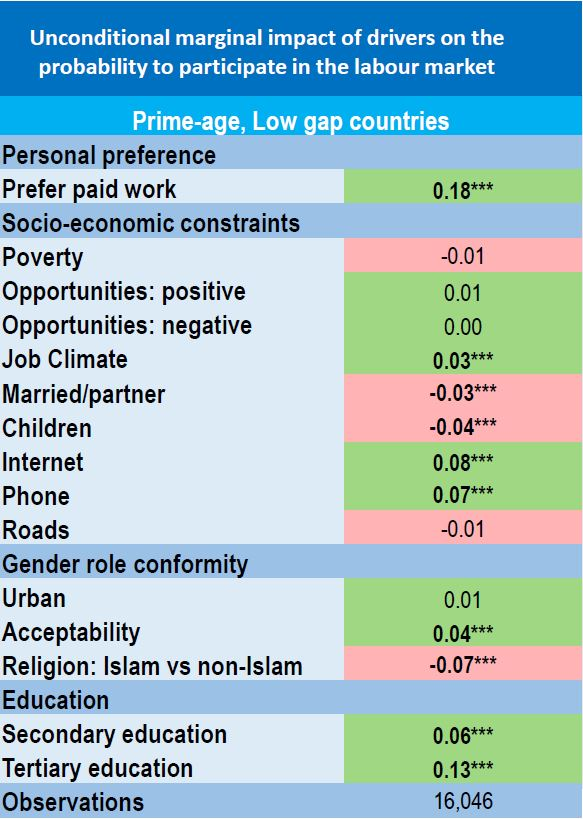
\includegraphics[width=70mm,keepaspectratio,height=0.6\textheight]{Figures/uncond_margins}
	\label{table:unconditional_marginal_effects}
\end{figure}

These baseline results highlight that a woman's participation is, among other things, very much a function of her ability to balance her role as a caregiver in the household with the demands of the workplace. A woman's role in the household and thus her preference and decision (even the freedom to choose) to participate in the labour market, are determined by social norms. The gender roles that arise from social norms vary across regions, but also vary according to the different traditional values held within different localities (urban vs rural), religions and even individual households.  

\subsection{Life-cycle effects}
To account for the various circumstances women face at different points in their lives, this section examines the differential life-cycle affects of the fundamental drivers across age groups and regions to account for the various circumstances women face at different points in their lives. 

First, the effects of socio-economic constraints on the probability to participate vary widely by age (Figure ~\ref{fig:constraints}) despite region. Poverty, for instance, follows a concave shape in effect as it increases the probability to participate for youth and even more-so for the elderly but has a slight negative affect among prime-age women. Living in an urban area has a positive affect among youth and prime-age women, but significantly reduces the probability to participate among elderly women. The perception of job opportunities has a positive affect on participation among prime and elderly but unexpectedly reduces the probability for youth. These findings highlight the varying degrees in which socio-economic constraints can affect the decision to participate for women depending on their life-cycle circumstances. 

\begin{figure}[htb]
	\centering
	\caption{Life-cycle effects: socio-economic constraints}
	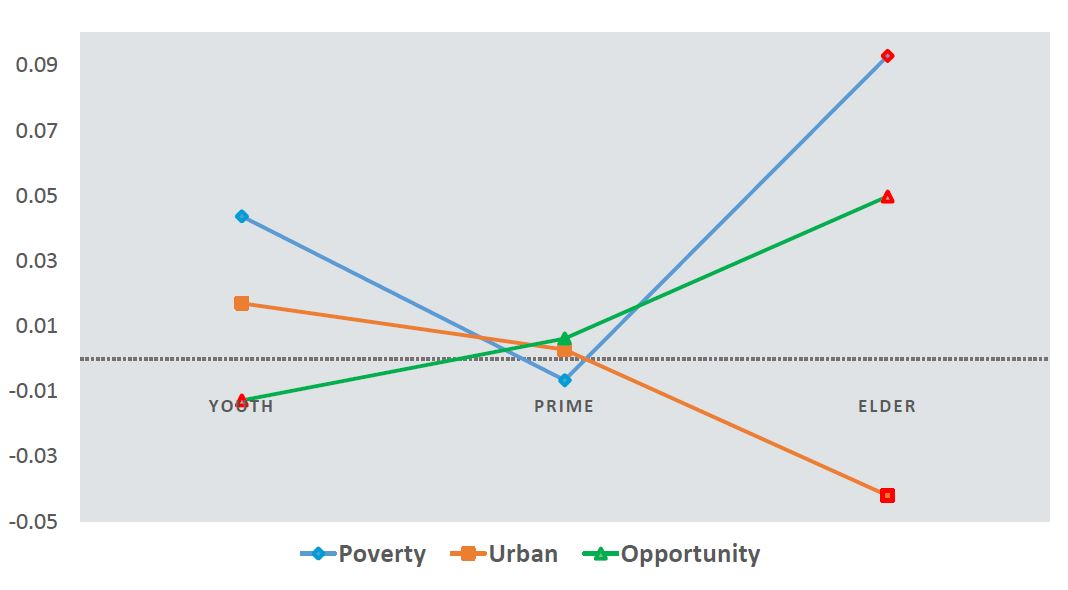
\includegraphics[width=120mm,keepaspectratio,height=0.6\textheight]{Figures/socioecon}
	\label{fig:constraints}
\end{figure}

This affect is also demonstrated by the varying challenges women face at different points in their lives, as reported in the survey, and to what extent these challenges affect their probability to participate (Figure ~\ref{fig:challenges}). Youth and prime-age women in low-gap countries most frequently report 'work and family balance' and 'abuse, harassment, and discrimination' as the biggest challenge faced in the labour market, while elderly women most frequently report 'work and family balance' and 'unequal pay'. Yet, the actual challenges that significantly affect their probability to participate differs. Youth are most significantly negatively affected by 'lack of transportation' and 'work and family balance' while for prime-age women they are most significantly negatively affected by the challenges of 'lack of transportation' and 'family members don't approve'. For elderly women, no challenges were estimated to significantly affect their probability to participate.  


\begin{figure}[htb]
	\centering
	\caption{Life-cycle effects: challenges in the labour market}
	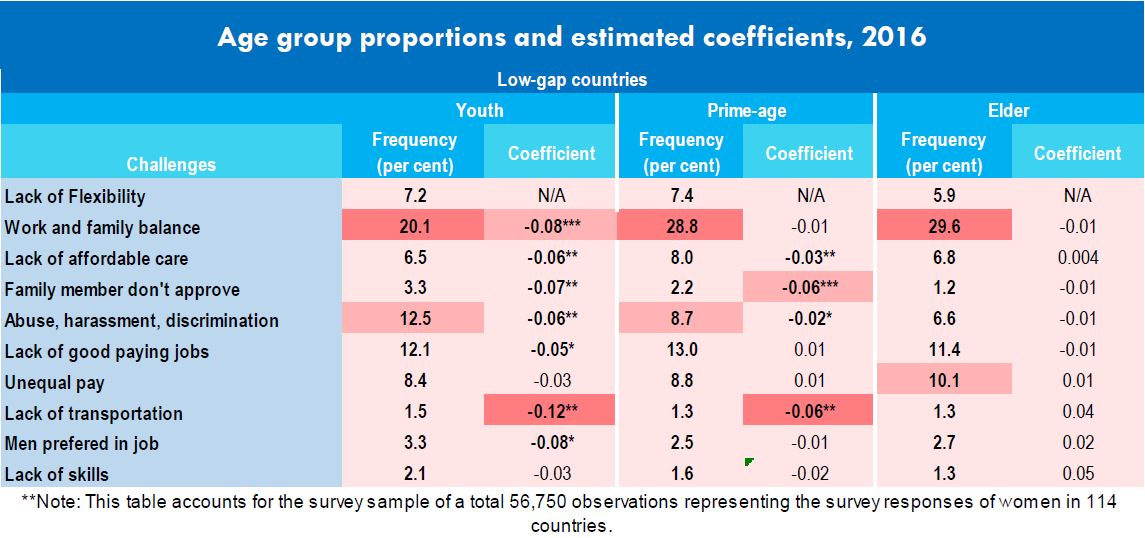
\includegraphics[width=140mm,keepaspectratio,height=0.6\textheight]{Figures/challenges}
	\label{fig:challenges}
\end{figure}

The life-cycle effects also differ across regions (Figure ~\ref{fig:marriage}). First, the general effects of partnership on the probability to participate follow a similar concave life-cycle pattern across the regions but at different magnitudes. Partnership increases the probability to participate for youth and elderly across all regions, while for prime-age women the effect is negative and to a significantly greater extent in high-gap countries. Overall, the probability to participate is higher in developing countries given the economic conditions of the region which induces a greater need to work. In general, the lower probabilities of participating among partnered prime-age women are likely due to two main reasons. The first is the economic stability that arises from a partner's income, reinforced by the 'male breadwinner' bias: the fact that the (male) 'breadwinner' is providing the household income reduces the economic imperative for a woman's labour market participation (in the case of developing countries, this effect is outweighed by economic necessity). The second and related reason is that economic stability enables social norms to confine women to more traditional roles within the household, i.e. shouldering a disproportionate burden of household responsibilities, which limits their choice and availability for paid work.

\begin{figure}[htb]
	\centering
	\caption{Life-cycle effects: partnership}
	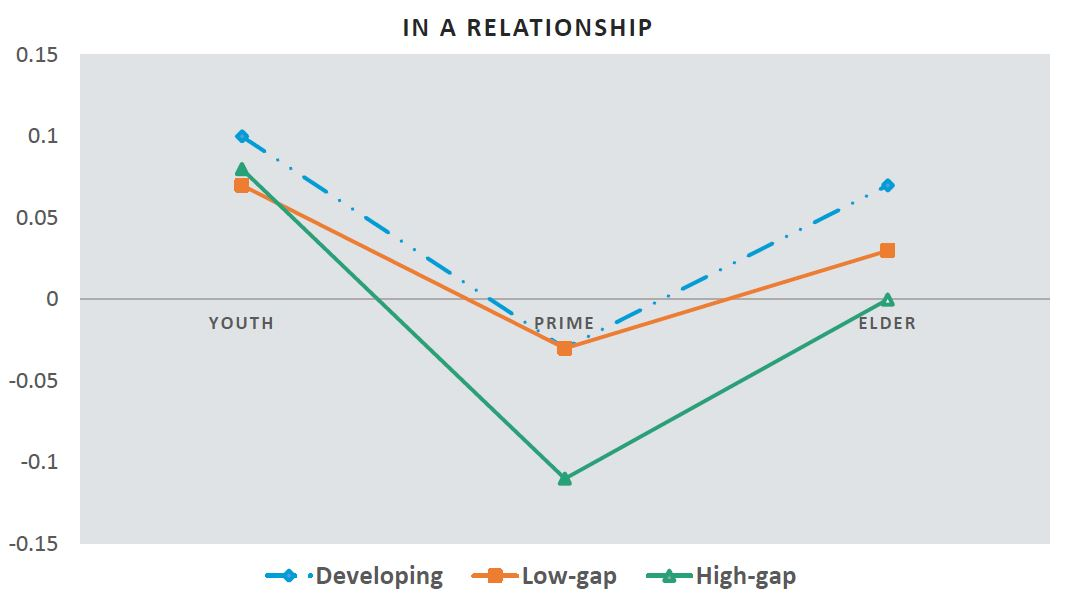
\includegraphics[width=120mm,keepaspectratio,height=0.6\textheight]{Figures/relationship}
	\label{fig:marriage}
\end{figure}

Lastly and most surprisingly, the life-cycle affects of education across the regions demonstrate divergent patterns (Figure ~\ref{fig:education} and ~\ref{fig:education2}). Youth women in developing countries face a negative probability to participate with secondary and tertiary education whereas in both low-gap and high-gap countries the affect is positive and increases for women with tertiary education. For prime-age women across all regions, both secondary and tertiary education increases the probability to work. This is similarly the case for elderly women in low-gap and high-gap countries, however, for elderly women in developing countries this increase in probability is particularly high for secondary education and negative for tertiary education. 

These results potentially suggest that the education variables for developing countries is likely to be picking up on other factors unaccounted for by the model. Hence, it is one possibility to consider that the effect of education on the probability to participate in the labour market is a function of the different weights given to the income and substitution effects. The substitution effect reflects the larger opportunity cost of staying at home as potential labour income rises with higher education, thereby encouraging participation. The income effect, in contrast, occurs when the economic needs of the family can be met with a lower rate of participation, so that more of a woman's time can be devoted to fulfilling traditional gender roles. The impact of education on participation might also capture more than just the balance between the income and substitution effects. Indeed, the level of education a woman can attain is, to a certain degree, influenced by other factors. A higher level of education could actually be an indicator that a woman's gender role and socio-economic conditions are generally more conducive to participation. In that case, the direct impact of higher education is likely to be overestimated.

\begin{figure}[htb]
	\centering
	\caption{Life-cycle effects: secondary education}
	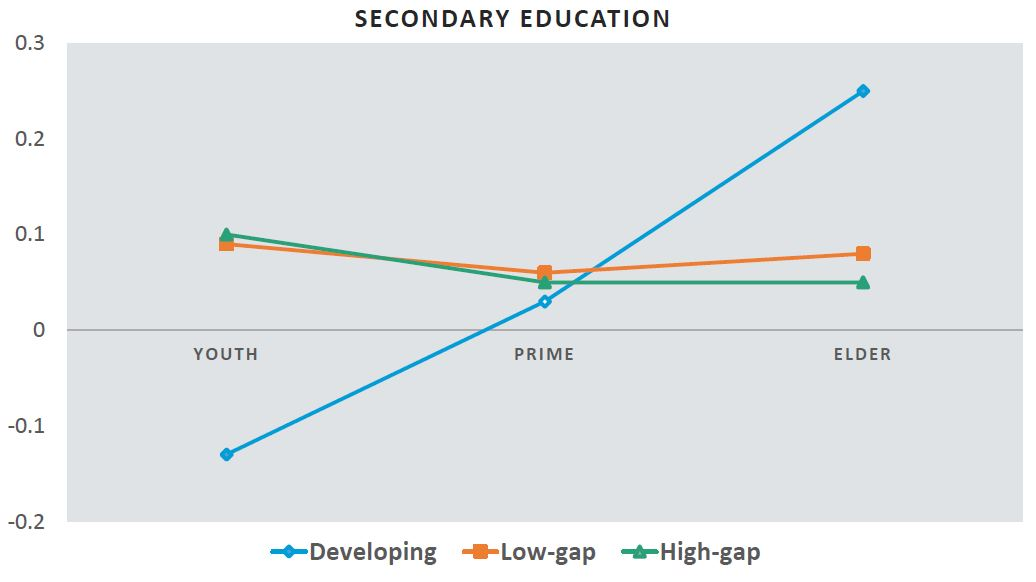
\includegraphics[width=120mm,keepaspectratio,height=0.6\textheight]{Figures/education}
	\label{fig:education}
\end{figure}

\begin{figure}[htb]
	\centering
	\caption{Life-cycle effects: tertiary education}
	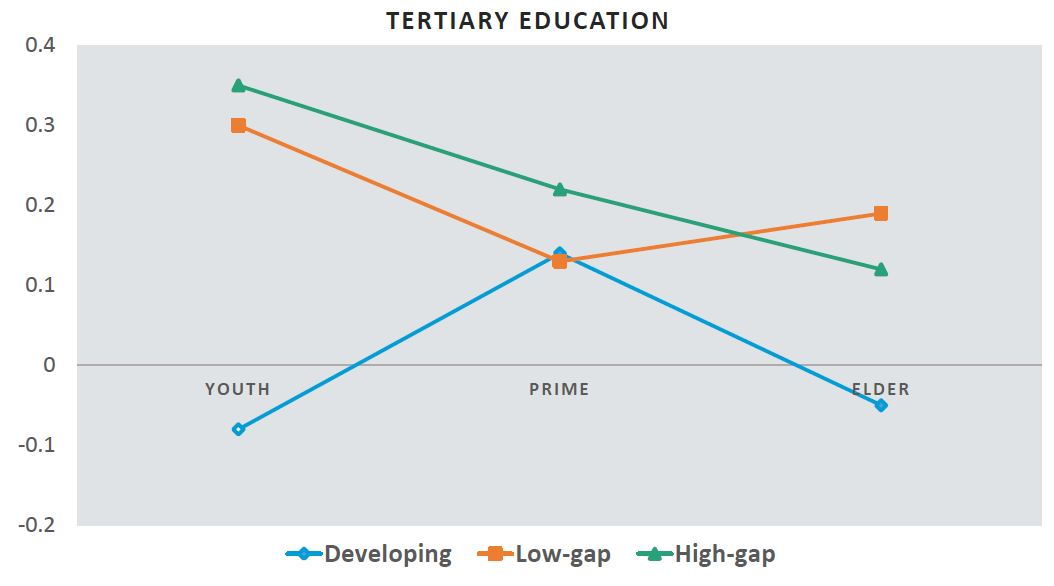
\includegraphics[width=120mm,keepaspectratio,height=0.6\textheight]{Figures/education_2}
	\label{fig:education2}
\end{figure}



\subsection{Planned future work}
For the future, some further analysis is planned. For instance, the result that poverty strongly increases the probability to participate for elderly women is very startling. One aim is to investigate whether this result varies according to the type of welfare state, providing potentially important policy conclusions.

Second, the current analysis uses the observed labour force participation gap in countries as a proxy to differentiate whether women's participation in a country is viewed favourably or not. An alternative measure would be the average response of men to the question whether women should pursue paid work form the ILO-Gallup survey. The latter has the advantage that it is a direct measure instead of a proxy, but has the disadvantage that the measure is quite noisy due to small sample size and that it only measures part of the environment that shapes women's participation. Nevertheless, it is a useful cross-check.

%

















\section{Robustness checks}
Robustness checks
\section{Conclusion}\label{sec:conclusion}

In conclusion, this paper provide strong evidence that a woman's preference to work has a significant positive effect on participation. However, preferences are a function of a range of factors, including women's life-cycle circumstances, their socio-economic conditions, their gender roles and the conditions of the local labour market of the region. Additionally, a number of socio-economic constraints also influence the probability to participate. Importantly, the influence of these constraints is not the same for all women, but varies according to the life cycle and to country characteristics. This has important policy implications, as it is necessary to know the constraints that women face before designing policies aiming at reducing gender gaps in the labour market.

\bibliographystyle{chicago}
\bibliography{ref_women_participation}

\appendix
\section{Appendix}


%\begin{table}\footnotesize
%	\caption{Table of coefficients}
	\documentclass[]{article}\pagestyle{empty}\begin{document}
\begin{center}
\begin{tabular}{lccccccccc}
\hline \noalign{\smallskip}age=0 cat=1 &  &  &  &  &  &  &  &  & \\
\noalign{\smallskip}\hline \noalign{\smallskip}1.PFW & -0.29 & -0.26 & 0.12 & 0.18 & 0.03 & 0.54 & 0.09 & -0.22 & 0.49\\
 & \begin{footnotesize}(0.26)\end{footnotesize} & \begin{footnotesize}(0.24)\end{footnotesize} & \begin{footnotesize}(0.18)\end{footnotesize} & \begin{footnotesize}(0.29)\end{footnotesize} & \begin{footnotesize}(0.24)\end{footnotesize} & \begin{footnotesize}(0.06)**\end{footnotesize} & \begin{footnotesize}(0.56)\end{footnotesize} & \begin{footnotesize}(0.29)\end{footnotesize} & \begin{footnotesize}(0.05)**\end{footnotesize}\\
\noalign{\smallskip}HHM & -0.06 & -0.12 & -0.03 & -0.01 & -0.08 & 0.04 & -0.19 & -0.08 & 0.16\\
 & \begin{footnotesize}(0.03)*\end{footnotesize} & \begin{footnotesize}(0.05)*\end{footnotesize} & \begin{footnotesize}(0.04)\end{footnotesize} & \begin{footnotesize}(0.03)\end{footnotesize} & \begin{footnotesize}(0.06)\end{footnotesize} & \begin{footnotesize}(0.03)\end{footnotesize} & \begin{footnotesize}(0.09)*\end{footnotesize} & \begin{footnotesize}(0.12)\end{footnotesize} & \begin{footnotesize}(0.05)**\end{footnotesize}\\
\noalign{\smallskip}c.HHM\#c.HHM & 0.01 & 0.01 & 0.00 & 0.00 & 0.01 & -0.01 & 0.01 & 0.02 & -0.02\\
 & \begin{footnotesize}(0.00)*\end{footnotesize} & \begin{footnotesize}(0.01)\end{footnotesize} & \begin{footnotesize}(0.00)\end{footnotesize} & \begin{footnotesize}(0.00)\end{footnotesize} & \begin{footnotesize}(0.01)*\end{footnotesize} & \begin{footnotesize}(0.00)\end{footnotesize} & \begin{footnotesize}(0.01)\end{footnotesize} & \begin{footnotesize}(0.02)\end{footnotesize} & \begin{footnotesize}(0.01)**\end{footnotesize}\\
\noalign{\smallskip}1.RLS & 0.27 & 0.15 & 0.25 & -0.12 & -0.35 & -0.28 & 0.18 & 0.16 & 0.05\\
 & \begin{footnotesize}(0.06)**\end{footnotesize} & \begin{footnotesize}(0.06)*\end{footnotesize} & \begin{footnotesize}(0.07)**\end{footnotesize} & \begin{footnotesize}(0.05)*\end{footnotesize} & \begin{footnotesize}(0.10)**\end{footnotesize} & \begin{footnotesize}(0.04)**\end{footnotesize} & \begin{footnotesize}(0.11)\end{footnotesize} & \begin{footnotesize}(0.05)**\end{footnotesize} & \begin{footnotesize}(0.05)\end{footnotesize}\\
\noalign{\smallskip}2bn.EDU & -0.38 & 0.13 & 0.43 & 0.08 & 0.10 & 0.16 & 0.87 & 0.04 & 0.37\\
 & \begin{footnotesize}(0.06)**\end{footnotesize} & \begin{footnotesize}(0.06)*\end{footnotesize} & \begin{footnotesize}(0.15)**\end{footnotesize} & \begin{footnotesize}(0.06)\end{footnotesize} & \begin{footnotesize}(0.04)*\end{footnotesize} & \begin{footnotesize}(0.04)**\end{footnotesize} & \begin{footnotesize}(0.24)**\end{footnotesize} & \begin{footnotesize}(0.10)\end{footnotesize} & \begin{footnotesize}(0.06)**\end{footnotesize}\\
\noalign{\smallskip}3.EDU & -0.21 & 0.82 & 0.58 & 0.52 & 0.45 & 0.52 & -0.09 & 0.26 & 0.65\\
 & \begin{footnotesize}(0.31)\end{footnotesize} & \begin{footnotesize}(0.11)**\end{footnotesize} & \begin{footnotesize}(0.29)*\end{footnotesize} & \begin{footnotesize}(0.16)**\end{footnotesize} & \begin{footnotesize}(0.06)**\end{footnotesize} & \begin{footnotesize}(0.05)**\end{footnotesize} & \begin{footnotesize}(0.50)\end{footnotesize} & \begin{footnotesize}(0.16)\end{footnotesize} & \begin{footnotesize}(0.08)**\end{footnotesize}\\
\noalign{\smallskip}1.CHD & 0.12 & 0.04 & -0.18 & 0.17 & -0.03 & -0.12 & -0.04 & 0.01 & -0.05\\
 & \begin{footnotesize}(0.08)\end{footnotesize} & \begin{footnotesize}(0.06)\end{footnotesize} & \begin{footnotesize}(0.06)**\end{footnotesize} & \begin{footnotesize}(0.09)\end{footnotesize} & \begin{footnotesize}(0.03)\end{footnotesize} & \begin{footnotesize}(0.03)**\end{footnotesize} & \begin{footnotesize}(0.13)\end{footnotesize} & \begin{footnotesize}(0.07)\end{footnotesize} & \begin{footnotesize}(0.06)\end{footnotesize}\\
\noalign{\smallskip}1.PVT & 0.25 & 0.23 & 0.01 & 0.15 & 0.40 & 0.24 & 0.32 & 0.10 & 0.05\\
 & \begin{footnotesize}(0.06)**\end{footnotesize} & \begin{footnotesize}(0.06)**\end{footnotesize} & \begin{footnotesize}(0.14)\end{footnotesize} & \begin{footnotesize}(0.05)**\end{footnotesize} & \begin{footnotesize}(0.10)**\end{footnotesize} & \begin{footnotesize}(0.06)**\end{footnotesize} & \begin{footnotesize}(0.11)**\end{footnotesize} & \begin{footnotesize}(0.05)\end{footnotesize} & \begin{footnotesize}(0.05)\end{footnotesize}\\
\noalign{\smallskip}1.COM & 0.30 & -0.55 & 0.14 & 0.14 & -0.24 & 0.20 & 0.19 & 0.28 & 0.28\\
 & \begin{footnotesize}(0.06)**\end{footnotesize} & \begin{footnotesize}(0.26)*\end{footnotesize} & \begin{footnotesize}(0.09)\end{footnotesize} & \begin{footnotesize}(0.05)**\end{footnotesize} & \begin{footnotesize}(0.16)\end{footnotesize} & \begin{footnotesize}(0.05)**\end{footnotesize} & \begin{footnotesize}(0.11)\end{footnotesize} & \begin{footnotesize}(0.10)**\end{footnotesize} & \begin{footnotesize}(0.07)**\end{footnotesize}\\
\noalign{\smallskip}1.URB & -0.53 & 0.08 & 0.04 & 0.05 & 0.05 & -0.11 & -0.55 & -0.44 & -0.04\\
 & \begin{footnotesize}(0.24)*\end{footnotesize} & \begin{footnotesize}(0.05)\end{footnotesize} & \begin{footnotesize}(0.06)\end{footnotesize} & \begin{footnotesize}(0.06)\end{footnotesize} & \begin{footnotesize}(0.03)\end{footnotesize} & \begin{footnotesize}(0.06)\end{footnotesize} & \begin{footnotesize}(0.22)*\end{footnotesize} & \begin{footnotesize}(0.09)**\end{footnotesize} & \begin{footnotesize}(0.05)\end{footnotesize}\\
\noalign{\smallskip}1bn.OPP & 0.06 & -0.15 & 0.10 & 0.02 & 0.41 & 0.13 & -0.23 & 0.12 & 0.11\\
 & \begin{footnotesize}(0.07)\end{footnotesize} & \begin{footnotesize}(0.06)*\end{footnotesize} & \begin{footnotesize}(0.07)\end{footnotesize} & \begin{footnotesize}(0.06)\end{footnotesize} & \begin{footnotesize}(0.12)**\end{footnotesize} & \begin{footnotesize}(0.04)**\end{footnotesize} & \begin{footnotesize}(0.21)\end{footnotesize} & \begin{footnotesize}(0.07)\end{footnotesize} & \begin{footnotesize}(0.07)\end{footnotesize}\\
\noalign{\smallskip}3.OPP & 0.07 & -0.04 & -0.11 & 0.10 & 0.02 & 0.04 & 0.09 & -0.05 & -0.01\\
 & \begin{footnotesize}(0.07)\end{footnotesize} & \begin{footnotesize}(0.06)\end{footnotesize} & \begin{footnotesize}(0.07)\end{footnotesize} & \begin{footnotesize}(0.06)\end{footnotesize} & \begin{footnotesize}(0.10)\end{footnotesize} & \begin{footnotesize}(0.04)\end{footnotesize} & \begin{footnotesize}(0.23)\end{footnotesize} & \begin{footnotesize}(0.05)\end{footnotesize} & \begin{footnotesize}(0.06)\end{footnotesize}\\
\noalign{\smallskip}4.OPP & 0.05 & -0.13 & -0.07 & -0.07 & 0.13 & -0.20 & 0.19 & -0.15 & -0.14\\
 & \begin{footnotesize}(0.13)\end{footnotesize} & \begin{footnotesize}(0.14)\end{footnotesize} & \begin{footnotesize}(0.16)\end{footnotesize} & \begin{footnotesize}(0.10)\end{footnotesize} & \begin{footnotesize}(0.20)\end{footnotesize} & \begin{footnotesize}(0.08)*\end{footnotesize} & \begin{footnotesize}(0.28)\end{footnotesize} & \begin{footnotesize}(0.09)\end{footnotesize} & \begin{footnotesize}(0.11)\end{footnotesize}\\
\noalign{\smallskip}2bn.CHG & -0.32 & -0.14 & -0.33 & 0.22 & -0.03 & -0.09 & 0.18 & 0.21 & -0.09\\
 & \begin{footnotesize}(0.14)*\end{footnotesize} & \begin{footnotesize}(0.10)\end{footnotesize} & \begin{footnotesize}(0.11)**\end{footnotesize} & \begin{footnotesize}(0.24)\end{footnotesize} & \begin{footnotesize}(0.06)\end{footnotesize} & \begin{footnotesize}(0.06)\end{footnotesize} & \begin{footnotesize}(0.45)\end{footnotesize} & \begin{footnotesize}(0.22)\end{footnotesize} & \begin{footnotesize}(0.10)\end{footnotesize}\\
\noalign{\smallskip}3.CHG & -0.28 & -0.18 & -0.20 & 0.46 & -0.06 & -0.15 & -0.07 & -0.02 & -0.14\\
 & \begin{footnotesize}(0.14)\end{footnotesize} & \begin{footnotesize}(0.13)\end{footnotesize} & \begin{footnotesize}(0.13)\end{footnotesize} & \begin{footnotesize}(0.25)\end{footnotesize} & \begin{footnotesize}(0.07)\end{footnotesize} & \begin{footnotesize}(0.07)*\end{footnotesize} & \begin{footnotesize}(0.45)\end{footnotesize} & \begin{footnotesize}(0.25)\end{footnotesize} & \begin{footnotesize}(0.13)\end{footnotesize}\\
\noalign{\smallskip}4.CHG & -0.30 & -0.24 & -0.28 & 0.25 & -0.17 & -0.27 & -0.50 & 0.25 & -0.31\\
 & \begin{footnotesize}(0.16)\end{footnotesize} & \begin{footnotesize}(0.17)\end{footnotesize} & \begin{footnotesize}(0.14)*\end{footnotesize} & \begin{footnotesize}(0.27)\end{footnotesize} & \begin{footnotesize}(0.11)\end{footnotesize} & \begin{footnotesize}(0.09)**\end{footnotesize} & \begin{footnotesize}(0.50)\end{footnotesize} & \begin{footnotesize}(0.41)\end{footnotesize} & \begin{footnotesize}(0.17)\end{footnotesize}\\
\noalign{\smallskip}5.CHG & -0.23 & -0.19 & -0.25 & 0.40 & -0.02 & -0.15 & -0.42 & 0.16 & -0.08\\
 & \begin{footnotesize}(0.14)\end{footnotesize} & \begin{footnotesize}(0.11)\end{footnotesize} & \begin{footnotesize}(0.13)*\end{footnotesize} & \begin{footnotesize}(0.25)\end{footnotesize} & \begin{footnotesize}(0.07)\end{footnotesize} & \begin{footnotesize}(0.08)*\end{footnotesize} & \begin{footnotesize}(0.44)\end{footnotesize} & \begin{footnotesize}(0.26)\end{footnotesize} & \begin{footnotesize}(0.13)\end{footnotesize}\\
\noalign{\smallskip}6.CHG & -0.25 & -0.09 & -0.20 & 0.57 & -0.02 & 0.00 & -0.60 & 0.05 & -0.08\\
 & \begin{footnotesize}(0.15)\end{footnotesize} & \begin{footnotesize}(0.12)\end{footnotesize} & \begin{footnotesize}(0.12)\end{footnotesize} & \begin{footnotesize}(0.28)*\end{footnotesize} & \begin{footnotesize}(0.07)\end{footnotesize} & \begin{footnotesize}(0.07)\end{footnotesize} & \begin{footnotesize}(0.50)\end{footnotesize} & \begin{footnotesize}(0.23)\end{footnotesize} & \begin{footnotesize}(0.11)\end{footnotesize}\\
\noalign{\smallskip}7.CHG & -0.20 & -0.21 & 0.04 & 1.25 & 0.07 & 0.04 & 0.22 & 0.07 & 0.11\\
 & \begin{footnotesize}(0.19)\end{footnotesize} & \begin{footnotesize}(0.13)\end{footnotesize} & \begin{footnotesize}(0.16)\end{footnotesize} & \begin{footnotesize}(0.60)*\end{footnotesize} & \begin{footnotesize}(0.08)\end{footnotesize} & \begin{footnotesize}(0.09)\end{footnotesize} & \begin{footnotesize}(0.54)\end{footnotesize} & \begin{footnotesize}(0.26)\end{footnotesize} & \begin{footnotesize}(0.13)\end{footnotesize}\\
\noalign{\smallskip}8.CHG & -0.38 & -0.45 & -0.46 & -0.83 & 0.07 & -0.14 & -0.72 & 0.78 & -0.06\\
 & \begin{footnotesize}(0.26)\end{footnotesize} & \begin{footnotesize}(0.25)\end{footnotesize} & \begin{footnotesize}(0.20)*\end{footnotesize} & \begin{footnotesize}(0.46)\end{footnotesize} & \begin{footnotesize}(0.20)\end{footnotesize} & \begin{footnotesize}(0.11)\end{footnotesize} & \begin{footnotesize}(0.62)\end{footnotesize} & \begin{footnotesize}(0.48)\end{footnotesize} & \begin{footnotesize}(0.18)\end{footnotesize}\\
\noalign{\smallskip}9.CHG & -0.25 & -0.35 & -0.12 & 0.82 & 0.04 & -0.14 & -0.12 & 0.83 & 0.07\\
 & \begin{footnotesize}(0.21)\end{footnotesize} & \begin{footnotesize}(0.17)*\end{footnotesize} & \begin{footnotesize}(0.19)\end{footnotesize} & \begin{footnotesize}(0.41)*\end{footnotesize} & \begin{footnotesize}(0.11)\end{footnotesize} & \begin{footnotesize}(0.14)\end{footnotesize} & \begin{footnotesize}(0.64)\end{footnotesize} & \begin{footnotesize}(0.35)*\end{footnotesize} & \begin{footnotesize}(0.18)\end{footnotesize}\\
\noalign{\smallskip}10.CHG & -0.31 & 0.34 & -0.24 & 0.62 & -0.29 & -0.02 & -0.68 & -0.51 & 0.35\\
 & \begin{footnotesize}(0.18)\end{footnotesize} & \begin{footnotesize}(0.21)\end{footnotesize} & \begin{footnotesize}(0.18)\end{footnotesize} & \begin{footnotesize}(0.31)*\end{footnotesize} & \begin{footnotesize}(0.12)*\end{footnotesize} & \begin{footnotesize}(0.12)\end{footnotesize} & \begin{footnotesize}(0.51)\end{footnotesize} & \begin{footnotesize}(0.38)\end{footnotesize} & \begin{footnotesize}(0.19)\end{footnotesize}\\
\noalign{\smallskip}97.CHG & -0.37 & -0.02 & -0.22 & 0.20 & 0.07 & -0.08 & -0.95 & -0.13 & -0.09\\
 & \begin{footnotesize}(0.16)*\end{footnotesize} & \begin{footnotesize}(0.13)\end{footnotesize} & \begin{footnotesize}(0.15)\end{footnotesize} & \begin{footnotesize}(0.30)\end{footnotesize} & \begin{footnotesize}(0.08)\end{footnotesize} & \begin{footnotesize}(0.08)\end{footnotesize} & \begin{footnotesize}(0.54)\end{footnotesize} & \begin{footnotesize}(0.24)\end{footnotesize} & \begin{footnotesize}(0.13)\end{footnotesize}\\
\noalign{\smallskip}98.CHG & -0.26 & -0.24 & -0.38 & 0.23 & -0.13 & -0.22 & -0.34 & -0.16 & -0.08\\
 & \begin{footnotesize}(0.14)\end{footnotesize} & \begin{footnotesize}(0.11)*\end{footnotesize} & \begin{footnotesize}(0.12)**\end{footnotesize} & \begin{footnotesize}(0.24)\end{footnotesize} & \begin{footnotesize}(0.07)\end{footnotesize} & \begin{footnotesize}(0.07)**\end{footnotesize} & \begin{footnotesize}(0.43)\end{footnotesize} & \begin{footnotesize}(0.23)\end{footnotesize} & \begin{footnotesize}(0.12)\end{footnotesize}\\
\noalign{\smallskip}1.REL & -0.28 & -0.32 & -0.37 & -0.21 & -0.26 & -0.17 & 0.00 & -0.29 & -0.02\\
 & \begin{footnotesize}(0.08)**\end{footnotesize} & \begin{footnotesize}(0.10)**\end{footnotesize} & \begin{footnotesize}(0.16)*\end{footnotesize} & \begin{footnotesize}(0.07)**\end{footnotesize} & \begin{footnotesize}(0.07)**\end{footnotesize} & \begin{footnotesize}(0.11)\end{footnotesize} & \begin{footnotesize}(0.22)\end{footnotesize} & \begin{footnotesize}(0.13)*\end{footnotesize} & \begin{footnotesize}(0.16)\end{footnotesize}\\
\noalign{\smallskip}1.ACW & 0.17 & 0.01 & 0.00 & 0.05 & 0.13 & 0.18 & -0.02 & 0.23 & -0.03\\
 & \begin{footnotesize}(0.09)\end{footnotesize} & \begin{footnotesize}(0.11)\end{footnotesize} & \begin{footnotesize}(0.09)\end{footnotesize} & \begin{footnotesize}(0.07)\end{footnotesize} & \begin{footnotesize}(0.07)\end{footnotesize} & \begin{footnotesize}(0.05)**\end{footnotesize} & \begin{footnotesize}(0.15)\end{footnotesize} & \begin{footnotesize}(0.12)*\end{footnotesize} & \begin{footnotesize}(0.09)\end{footnotesize}\\
\noalign{\smallskip}1.RDS & 0.05 & 0.10 & -0.05 & -0.30 & -0.22 & -0.02 & 0.19 & -0.20 & -0.07\\
 & \begin{footnotesize}(0.07)\end{footnotesize} & \begin{footnotesize}(0.06)\end{footnotesize} & \begin{footnotesize}(0.06)\end{footnotesize} & \begin{footnotesize}(0.11)**\end{footnotesize} & \begin{footnotesize}(0.09)*\end{footnotesize} & \begin{footnotesize}(0.04)\end{footnotesize} & \begin{footnotesize}(0.13)\end{footnotesize} & \begin{footnotesize}(0.09)*\end{footnotesize} & \begin{footnotesize}(0.05)\end{footnotesize}\\
\noalign{\smallskip}1.TRP & 0.01 & 0.07 & 0.05 & 0.06 & -0.05 & 0.01 & -0.07 & -0.09 & -0.03\\
 & \begin{footnotesize}(0.07)\end{footnotesize} & \begin{footnotesize}(0.06)\end{footnotesize} & \begin{footnotesize}(0.06)\end{footnotesize} & \begin{footnotesize}(0.05)\end{footnotesize} & \begin{footnotesize}(0.03)\end{footnotesize} & \begin{footnotesize}(0.04)\end{footnotesize} & \begin{footnotesize}(0.13)\end{footnotesize} & \begin{footnotesize}(0.05)*\end{footnotesize} & \begin{footnotesize}(0.06)\end{footnotesize}\\
\noalign{\smallskip}LAW & -0.49 & -0.16 & -0.16 & -0.62 & 0.02 & 0.02 & -0.39 & -0.09 & 0.07\\
 & \begin{footnotesize}(0.32)\end{footnotesize} & \begin{footnotesize}(0.10)\end{footnotesize} & \begin{footnotesize}(0.11)\end{footnotesize} & \begin{footnotesize}(0.22)**\end{footnotesize} & \begin{footnotesize}(0.06)\end{footnotesize} & \begin{footnotesize}(0.07)\end{footnotesize} & \begin{footnotesize}(0.23)\end{footnotesize} & \begin{footnotesize}(0.09)\end{footnotesize} & \begin{footnotesize}(0.11)\end{footnotesize}\\
\noalign{\smallskip}JCL & 0.19 & 0.19 & -0.27 & 0.27 & 0.14 & 0.03 & 0.62 & 0.21 & 0.15\\
 & \begin{footnotesize}(0.07)*\end{footnotesize} & \begin{footnotesize}(0.07)**\end{footnotesize} & \begin{footnotesize}(0.17)\end{footnotesize} & \begin{footnotesize}(0.06)**\end{footnotesize} & \begin{footnotesize}(0.04)**\end{footnotesize} & \begin{footnotesize}(0.04)\end{footnotesize} & \begin{footnotesize}(0.15)**\end{footnotesize} & \begin{footnotesize}(0.06)**\end{footnotesize} & \begin{footnotesize}(0.07)*\end{footnotesize}\\
\noalign{\smallskip}1.PFW\#1.URB & 0.52 &  &  &  &  & 0.14 & 0.64 & 0.32 & \\
 & \begin{footnotesize}(0.24)*\end{footnotesize} & \begin{footnotesize}\end{footnotesize} & \begin{footnotesize}\end{footnotesize} & \begin{footnotesize}\end{footnotesize} & \begin{footnotesize}\end{footnotesize} & \begin{footnotesize}(0.07)\end{footnotesize} & \begin{footnotesize}(0.27)*\end{footnotesize} & \begin{footnotesize}(0.10)**\end{footnotesize} & \begin{footnotesize}\end{footnotesize}\\
\noalign{\smallskip}1.PFW\#c.LAW & 0.56 &  &  & 0.57 &  &  &  &  & \\
 & \begin{footnotesize}(0.33)\end{footnotesize} & \begin{footnotesize}\end{footnotesize} & \begin{footnotesize}\end{footnotesize} & \begin{footnotesize}(0.24)*\end{footnotesize} & \begin{footnotesize}\end{footnotesize} & \begin{footnotesize}\end{footnotesize} & \begin{footnotesize}\end{footnotesize} & \begin{footnotesize}\end{footnotesize} & \begin{footnotesize}\end{footnotesize}\\
\noalign{\smallskip}1.PFW\#1.COM &  & 0.64 &  &  & 0.39 &  &  &  & \\
 & \begin{footnotesize}\end{footnotesize} & \begin{footnotesize}(0.27)*\end{footnotesize} & \begin{footnotesize}\end{footnotesize} & \begin{footnotesize}\end{footnotesize} & \begin{footnotesize}(0.17)*\end{footnotesize} & \begin{footnotesize}\end{footnotesize} & \begin{footnotesize}\end{footnotesize} & \begin{footnotesize}\end{footnotesize} & \begin{footnotesize}\end{footnotesize}\\
\noalign{\smallskip}1.PFW\#c.JCL &  &  & 0.32 &  &  &  &  &  & \\
 & \begin{footnotesize}\end{footnotesize} & \begin{footnotesize}\end{footnotesize} & \begin{footnotesize}(0.19)\end{footnotesize} & \begin{footnotesize}\end{footnotesize} & \begin{footnotesize}\end{footnotesize} & \begin{footnotesize}\end{footnotesize} & \begin{footnotesize}\end{footnotesize} & \begin{footnotesize}\end{footnotesize} & \begin{footnotesize}\end{footnotesize}\\
\noalign{\smallskip}1.PFW\#2bn.EDU &  &  & -0.05 &  &  &  &  & 0.37 & \\
 & \begin{footnotesize}\end{footnotesize} & \begin{footnotesize}\end{footnotesize} & \begin{footnotesize}(0.16)\end{footnotesize} & \begin{footnotesize}\end{footnotesize} & \begin{footnotesize}\end{footnotesize} & \begin{footnotesize}\end{footnotesize} & \begin{footnotesize}\end{footnotesize} & \begin{footnotesize}(0.11)**\end{footnotesize} & \begin{footnotesize}\end{footnotesize}\\
\noalign{\smallskip}1.PFW\#3.EDU &  &  & 0.54 &  &  &  &  & 0.37 & \\
 & \begin{footnotesize}\end{footnotesize} & \begin{footnotesize}\end{footnotesize} & \begin{footnotesize}(0.32)\end{footnotesize} & \begin{footnotesize}\end{footnotesize} & \begin{footnotesize}\end{footnotesize} & \begin{footnotesize}\end{footnotesize} & \begin{footnotesize}\end{footnotesize} & \begin{footnotesize}(0.17)*\end{footnotesize} & \begin{footnotesize}\end{footnotesize}\\
\noalign{\smallskip}1.PFW\#1.PVT &  &  & 0.26 &  & -0.44 & -0.14 &  &  & \\
 & \begin{footnotesize}\end{footnotesize} & \begin{footnotesize}\end{footnotesize} & \begin{footnotesize}(0.15)\end{footnotesize} & \begin{footnotesize}\end{footnotesize} & \begin{footnotesize}(0.10)**\end{footnotesize} & \begin{footnotesize}(0.07)*\end{footnotesize} & \begin{footnotesize}\end{footnotesize} & \begin{footnotesize}\end{footnotesize} & \begin{footnotesize}\end{footnotesize}\\
\noalign{\smallskip}1.PFW\#2bn.CHG &  &  &  & -0.18 &  &  & -0.81 & -0.11 & \\
 & \begin{footnotesize}\end{footnotesize} & \begin{footnotesize}\end{footnotesize} & \begin{footnotesize}\end{footnotesize} & \begin{footnotesize}(0.27)\end{footnotesize} & \begin{footnotesize}\end{footnotesize} & \begin{footnotesize}\end{footnotesize} & \begin{footnotesize}(0.56)\end{footnotesize} & \begin{footnotesize}(0.24)\end{footnotesize} & \begin{footnotesize}\end{footnotesize}\\
\noalign{\smallskip}1.PFW\#3.CHG &  &  &  & -0.59 &  &  & -0.48 & 0.06 & \\
 & \begin{footnotesize}\end{footnotesize} & \begin{footnotesize}\end{footnotesize} & \begin{footnotesize}\end{footnotesize} & \begin{footnotesize}(0.27)*\end{footnotesize} & \begin{footnotesize}\end{footnotesize} & \begin{footnotesize}\end{footnotesize} & \begin{footnotesize}(0.57)\end{footnotesize} & \begin{footnotesize}(0.28)\end{footnotesize} & \begin{footnotesize}\end{footnotesize}\\
\noalign{\smallskip}1.PFW\#4.CHG &  &  &  & -0.46 &  &  & 0.61 & -0.24 & \\
 & \begin{footnotesize}\end{footnotesize} & \begin{footnotesize}\end{footnotesize} & \begin{footnotesize}\end{footnotesize} & \begin{footnotesize}(0.30)\end{footnotesize} & \begin{footnotesize}\end{footnotesize} & \begin{footnotesize}\end{footnotesize} & \begin{footnotesize}(0.66)\end{footnotesize} & \begin{footnotesize}(0.47)\end{footnotesize} & \begin{footnotesize}\end{footnotesize}\\
\noalign{\smallskip}1.PFW\#5.CHG &  &  &  & -0.52 &  &  & -0.24 & -0.17 & \\
 & \begin{footnotesize}\end{footnotesize} & \begin{footnotesize}\end{footnotesize} & \begin{footnotesize}\end{footnotesize} & \begin{footnotesize}(0.27)\end{footnotesize} & \begin{footnotesize}\end{footnotesize} & \begin{footnotesize}\end{footnotesize} & \begin{footnotesize}(0.55)\end{footnotesize} & \begin{footnotesize}(0.28)\end{footnotesize} & \begin{footnotesize}\end{footnotesize}\\
\noalign{\smallskip}1.PFW\#6.CHG &  &  &  & -0.54 &  &  & 0.27 & -0.03 & \\
 & \begin{footnotesize}\end{footnotesize} & \begin{footnotesize}\end{footnotesize} & \begin{footnotesize}\end{footnotesize} & \begin{footnotesize}(0.31)\end{footnotesize} & \begin{footnotesize}\end{footnotesize} & \begin{footnotesize}\end{footnotesize} & \begin{footnotesize}(0.61)\end{footnotesize} & \begin{footnotesize}(0.26)\end{footnotesize} & \begin{footnotesize}\end{footnotesize}\\
\noalign{\smallskip}1.PFW\#7.CHG &  &  &  & -1.33 &  &  & -0.71 & 0.07 & \\
 & \begin{footnotesize}\end{footnotesize} & \begin{footnotesize}\end{footnotesize} & \begin{footnotesize}\end{footnotesize} & \begin{footnotesize}(0.62)*\end{footnotesize} & \begin{footnotesize}\end{footnotesize} & \begin{footnotesize}\end{footnotesize} & \begin{footnotesize}(0.75)\end{footnotesize} & \begin{footnotesize}(0.28)\end{footnotesize} & \begin{footnotesize}\end{footnotesize}\\
\noalign{\smallskip}1.PFW\#8.CHG &  &  &  & 0.22 &  &  & 0.29 & -0.58 & \\
 & \begin{footnotesize}\end{footnotesize} & \begin{footnotesize}\end{footnotesize} & \begin{footnotesize}\end{footnotesize} & \begin{footnotesize}(0.51)\end{footnotesize} & \begin{footnotesize}\end{footnotesize} & \begin{footnotesize}\end{footnotesize} & \begin{footnotesize}(0.85)\end{footnotesize} & \begin{footnotesize}(0.55)\end{footnotesize} & \begin{footnotesize}\end{footnotesize}\\
\noalign{\smallskip}1.PFW\#9.CHG &  &  &  & -0.91 &  &  & 0.14 & -0.78 & \\
 & \begin{footnotesize}\end{footnotesize} & \begin{footnotesize}\end{footnotesize} & \begin{footnotesize}\end{footnotesize} & \begin{footnotesize}(0.45)*\end{footnotesize} & \begin{footnotesize}\end{footnotesize} & \begin{footnotesize}\end{footnotesize} & \begin{footnotesize}(0.91)\end{footnotesize} & \begin{footnotesize}(0.38)*\end{footnotesize} & \begin{footnotesize}\end{footnotesize}\\
\noalign{\smallskip}1.PFW\#10.CHG &  &  &  & -0.63 &  &  & 0.05 & 0.82 & \\
 & \begin{footnotesize}\end{footnotesize} & \begin{footnotesize}\end{footnotesize} & \begin{footnotesize}\end{footnotesize} & \begin{footnotesize}(0.35)\end{footnotesize} & \begin{footnotesize}\end{footnotesize} & \begin{footnotesize}\end{footnotesize} & \begin{footnotesize}(0.72)\end{footnotesize} & \begin{footnotesize}(0.43)\end{footnotesize} & \begin{footnotesize}\end{footnotesize}\\
\noalign{\smallskip}1.PFW\#97.CHG &  &  &  & -0.42 &  &  & 0.22 & 0.12 & \\
 & \begin{footnotesize}\end{footnotesize} & \begin{footnotesize}\end{footnotesize} & \begin{footnotesize}\end{footnotesize} & \begin{footnotesize}(0.33)\end{footnotesize} & \begin{footnotesize}\end{footnotesize} & \begin{footnotesize}\end{footnotesize} & \begin{footnotesize}(0.66)\end{footnotesize} & \begin{footnotesize}(0.26)\end{footnotesize} & \begin{footnotesize}\end{footnotesize}\\
\noalign{\smallskip}1.PFW\#98.CHG &  &  &  & -0.25 &  &  & -0.46 & 0.15 & \\
 & \begin{footnotesize}\end{footnotesize} & \begin{footnotesize}\end{footnotesize} & \begin{footnotesize}\end{footnotesize} & \begin{footnotesize}(0.26)\end{footnotesize} & \begin{footnotesize}\end{footnotesize} & \begin{footnotesize}\end{footnotesize} & \begin{footnotesize}(0.55)\end{footnotesize} & \begin{footnotesize}(0.26)\end{footnotesize} & \begin{footnotesize}\end{footnotesize}\\
\noalign{\smallskip}1.PFW\#1.RDS &  &  &  & 0.32 & 0.21 &  &  & 0.16 & \\
 & \begin{footnotesize}\end{footnotesize} & \begin{footnotesize}\end{footnotesize} & \begin{footnotesize}\end{footnotesize} & \begin{footnotesize}(0.12)**\end{footnotesize} & \begin{footnotesize}(0.09)*\end{footnotesize} & \begin{footnotesize}\end{footnotesize} & \begin{footnotesize}\end{footnotesize} & \begin{footnotesize}(0.10)\end{footnotesize} & \begin{footnotesize}\end{footnotesize}\\
\noalign{\smallskip}1.PFW\#c.HHM &  &  &  &  & 0.12 &  & 0.27 & 0.29 & \\
 & \begin{footnotesize}\end{footnotesize} & \begin{footnotesize}\end{footnotesize} & \begin{footnotesize}\end{footnotesize} & \begin{footnotesize}\end{footnotesize} & \begin{footnotesize}(0.06)\end{footnotesize} & \begin{footnotesize}\end{footnotesize} & \begin{footnotesize}(0.10)**\end{footnotesize} & \begin{footnotesize}(0.12)*\end{footnotesize} & \begin{footnotesize}\end{footnotesize}\\
\noalign{\smallskip}1.PFW\#c.HHM\#c.HHM &  &  &  &  & -0.01 &  & -0.02 & -0.04 & \\
 & \begin{footnotesize}\end{footnotesize} & \begin{footnotesize}\end{footnotesize} & \begin{footnotesize}\end{footnotesize} & \begin{footnotesize}\end{footnotesize} & \begin{footnotesize}(0.01)*\end{footnotesize} & \begin{footnotesize}\end{footnotesize} & \begin{footnotesize}(0.01)*\end{footnotesize} & \begin{footnotesize}(0.02)\end{footnotesize} & \begin{footnotesize}\end{footnotesize}\\
\noalign{\smallskip}1.PFW\#1.RLS &  &  &  &  & 0.22 &  &  &  & \\
 & \begin{footnotesize}\end{footnotesize} & \begin{footnotesize}\end{footnotesize} & \begin{footnotesize}\end{footnotesize} & \begin{footnotesize}\end{footnotesize} & \begin{footnotesize}(0.11)*\end{footnotesize} & \begin{footnotesize}\end{footnotesize} & \begin{footnotesize}\end{footnotesize} & \begin{footnotesize}\end{footnotesize} & \begin{footnotesize}\end{footnotesize}\\
\noalign{\smallskip}1.PFW\#1bn.OPP &  &  &  &  & -0.40 &  & 0.44 &  & \\
 & \begin{footnotesize}\end{footnotesize} & \begin{footnotesize}\end{footnotesize} & \begin{footnotesize}\end{footnotesize} & \begin{footnotesize}\end{footnotesize} & \begin{footnotesize}(0.13)**\end{footnotesize} & \begin{footnotesize}\end{footnotesize} & \begin{footnotesize}(0.27)\end{footnotesize} & \begin{footnotesize}\end{footnotesize} & \begin{footnotesize}\end{footnotesize}\\
\noalign{\smallskip}1.PFW\#3.OPP &  &  &  &  & -0.10 &  & 0.01 &  & \\
 & \begin{footnotesize}\end{footnotesize} & \begin{footnotesize}\end{footnotesize} & \begin{footnotesize}\end{footnotesize} & \begin{footnotesize}\end{footnotesize} & \begin{footnotesize}(0.10)\end{footnotesize} & \begin{footnotesize}\end{footnotesize} & \begin{footnotesize}(0.29)\end{footnotesize} & \begin{footnotesize}\end{footnotesize} & \begin{footnotesize}\end{footnotesize}\\
\noalign{\smallskip}1.PFW\#4.OPP &  &  &  &  & -0.16 &  & -0.49 &  & \\
 & \begin{footnotesize}\end{footnotesize} & \begin{footnotesize}\end{footnotesize} & \begin{footnotesize}\end{footnotesize} & \begin{footnotesize}\end{footnotesize} & \begin{footnotesize}(0.22)\end{footnotesize} & \begin{footnotesize}\end{footnotesize} & \begin{footnotesize}(0.41)\end{footnotesize} & \begin{footnotesize}\end{footnotesize} & \begin{footnotesize}\end{footnotesize}\\
\noalign{\smallskip}1.PFW\#1.REL &  &  &  &  &  & 0.15 & -0.42 &  & \\
 & \begin{footnotesize}\end{footnotesize} & \begin{footnotesize}\end{footnotesize} & \begin{footnotesize}\end{footnotesize} & \begin{footnotesize}\end{footnotesize} & \begin{footnotesize}\end{footnotesize} & \begin{footnotesize}(0.08)\end{footnotesize} & \begin{footnotesize}(0.23)\end{footnotesize} & \begin{footnotesize}\end{footnotesize} & \begin{footnotesize}\end{footnotesize}\\
\noalign{\smallskip}$N$ & 3,337 & 4,048 & 3,422 & 5,835 & 12,366 & 11,561 & 949 & 7,207 & 5,099\\
\noalign{\smallskip}\hline\end{tabular}\\
\end{center}
\end{document}

%\end{table}

\end{document}